\documentclass[12 pt]{article}
\usepackage[a4paper,top=3.5cm,bottom=3cm,left=3cm,right=3cm]{geometry}
\usepackage{graphicx} 
\usepackage{amssymb}
\usepackage{lmodern}
\usepackage{setspace}
\author{Vanessa Braglia}
\title{The swiss scientific social network}
\date{\today}

\onehalfspacing

\begin{document}
\fontfamily{lmr}\selectfont
\maketitle 
\newpage
\tableofcontents
\newpage
\section{Introduction}
A social network consists of a set of objects connected to each other by social relations. The best way to model social networks is using graphs (see an example in Figure 1): the objects (entities) are represented as nodes and the connections as edges between two different nodes. \\
\begin{figure} [h!]
\centering 
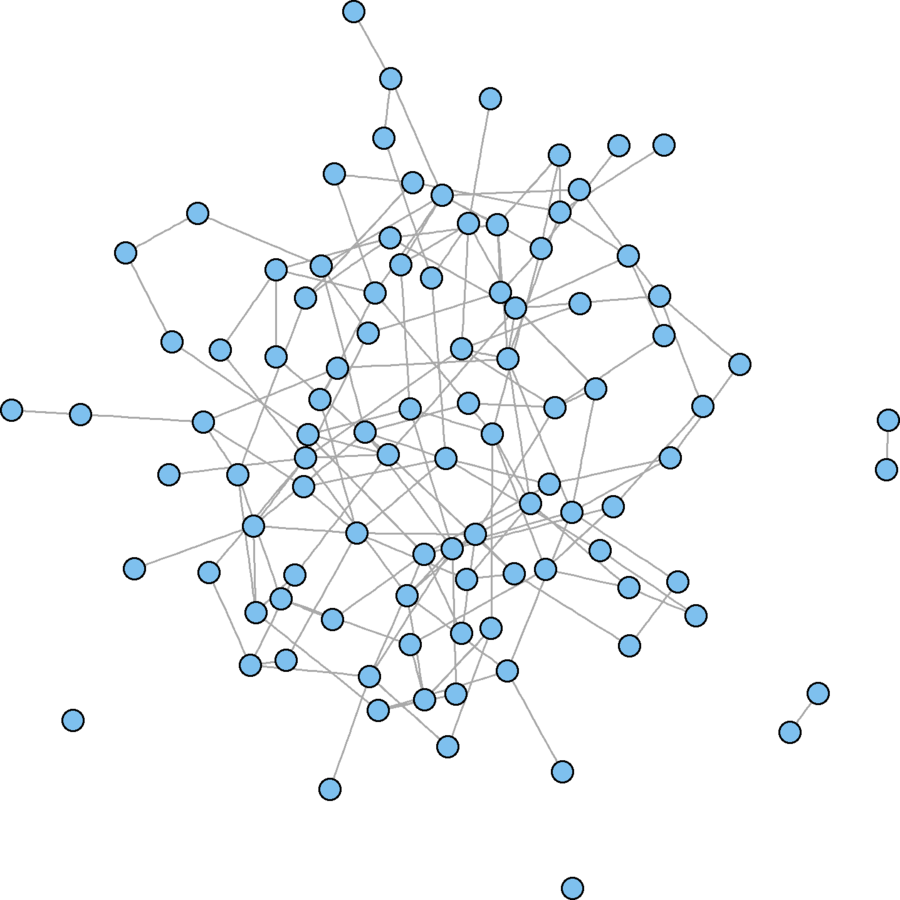
\includegraphics[scale=0.5]{graph.png}
\caption{Example of social network graph}
\end{figure}
\\
The goal of this project is to create a social network of computational science authors belonging to Swiss institutions and then analyze the relative graph.\\
The first step is retrieving all necessary information for the construction of the social network: names of the authors and relationships between each other. (aggiungere tutti gli argomenti delle conferenze) I crawled Pasc and Siam conferences and authors that did a conference together are considered coauthors.\\
The second step is the information analysis: I apply some methods such as PageRank algorithm (che consiste in..) and Graph Partitioning.
The results will provide an interesting picture of the different research scenarios in Switzerland and how they interact with each other.

\section{PageRank Algorithm}
PageRank (PR) is an algorithm used by Google Search to rank websites in their search engine results. PageRank was named after Larry Page,[1] one of the founders of Google. PageRank is a way of measuring the importance of website pages. According to Google:

    PageRank works by counting the number and quality of links to a page to determine a rough estimate of how important the website is. The underlying assumption is that more important websites are likely to receive more links from other websites.[2] 

It is not the only algorithm used by Google to order search engine results, but it is the first algorithm that was used by the company, and it is the best-known
One of the reasons why GoogleTM is such an effective search engine is the Page-RankTM algorithm developed by Google’s founders, Larry Page and Sergey Brin, when they were graduate students at Stanford University. PageRank is determined entirely by the link structure of the World Wide Web. It is recomputed about once a month and does not involve the actual content of any Web pages or individual queries. Then, for any particular query, Google finds the pages on the Web that match that query and lists those pages in the order of their PageRank. Imagine surfing the Web, going from page to page by randomly choosing an outgoing link from one page to get to the next. This can lead to dead ends at pages with no outgoing links, or cycles around cliques of interconnected pages. So, a certain fraction of the time, simply choose a random page from the Web. This theoretical random walk is known as a Markov chain or Markov process. The limiting probability that an infinitely dedicated random surfer visits any particular page is its PageRank. A page has high rank if other pages with high rank link to it.
Let W be the set of Web pages that can be reached by following a chain of hyperlinks starting at some root page and let n be the number of pages in W . For Google, the set W actually varies with time, but by the end of 2002, n was over 3 billion. Let G be the n-by-n connectivity matrix of a portion of the Web, that is gij = 1 if there is a hyperlink to page i from page j and zero otherwise. The matrix G can be huge, but it is very sparse. Its j-th column shows the links on the j -th page. The number of nonzeros in G is the total number of hyperlinks in W .
Let ri and cj be the row and column sums of G:

The quantities rj and cj are the in-degree and out-degree of the j-th page. Let p be the probability that the random walk follows a link. A typical value is p = 0.85. Then 1 − p is the probability that some arbitrary page is chosen and δ = (1 − p)/n is the probability that a particular random page is chosen. Let A be the n-by-n matrix whose elements are

Notice that A comes from scaling the connectivity matrix by its column sums. The j-th column is the probability of jumping from the j-th page to the other pages on the Web. If the j-th page is a dead end, that is has no out-links, then we assign a uniform probability of 1/n to all the elements in its column. Most of the elements of A are equal to δ, the probability of jumping from one page to another without following a link. If n = 4 · 109 and p = 0.85, then δ = 3.75 · 10−11. The matrix A is the transition probability matrix of the Markov chain. Its elements are all strictly between zero and one and its column sums are all equal to one. An important result in matrix theory known as the Perron–Frobenius theorem applies to such matrices. It concludes that a nonzero solution of the equation
\section{Graph Partitioning}

\section{Results}
\subsection{Information Retrieval}
\subsection{PageRank}
\subsection{Graph Partitioning}
\end{document}
